% 1. introduce metrics of RW
% - soft. eng., composition, code reuse, sep of concerns
% - parallelism levels
% 2. RW analyze
% - each tool
% - table
% 3. discussion
% - intra-task
% - performance model

%----------------------------
\subsection{Related work metrics}
%----------------------------
% 1. software engineering
% - components / service / module
% - sub-elements / tasks
% - separation of concerns when assembling 2 components, no need to
% know what each component does to commission itself
% 2. parallelism
% - node / SIMH
% - inter-component
% - inter-task
% - intra-task
% 3. formalism
% - formal model

Before introducing the related work of this paper, some analysis
metrics need to be introduced. These metrics are divided in three
sets: software engineering (SE) metrics, metrics related to the
parallelism level of commissionings, and metrics related to formal
aspects of commissionings. For each metric four levels will be
considered and presented in Table~\ref{tab:comparison}: (1) supported,
denoted with \checkmark, that counts for 3 points in the score; (2)
partially supported, denoted (\checkmark), that counts for 2 points;
(3) manually supported, denoted \emph{M}, meaning that the user may
code manually the given metric, and that counts 1 point; and finally
(4) not supported, denoted -.

\paragraph{Software engineering}
As introduced in the previous section, when automating distributed
software commissionings one important aspect is to promote software
engineering properties. Indeed, when different actors are involved in
a same given goal, software engineering techniques can help improving
separation of concerns (\ie code reuse, maintainability
etc.). Separation of concerns means that each actor is responsible for
her own specialism, \ie her own expertise domain. Such separation of
concerns is improved as soon as a modular or component-based approach
is adopted, \ie each actor could be responsible for one
component. Furthermore, component-based architectures are also equiped
with composition mechanisms that ease the interactions between the
different entities implemented by different actors. One additional
actor may also enter the picture to design this composition. We define
three SE metrics to compare the related work:
\begin{itemize}
\item \emph{component}: if the work (tool, framework or scientific
  contribution) offers a component-oriented (\eg services, modules)
  structure of commissionings;
\item \emph{tasks}: if the work (tool, framework or scientific
  contribution) offers a way to divide the commissioning of each
  component in sub-elements that we call \emph{tasks} and that promote
  even more a well structured procedural design;
\item \emph{separation of concerns}: if the work (tool, framework or
  scientific contribution) offers a way to build distributed software
  commissionings by composing each commissioning of individual
  components and while not needing to know their internal behaviors.
\end{itemize}

\paragraph{Parallelism level}
A second important aspect of distributed software commissioning that
has been introduced in the previous section is its efficiency and in
particular (in this paper) the level of parallelism offered by
commissioning tools and frameworks. We consider four metrics to
compare the related work:
\begin{itemize}
\item \emph{SIMH}: if the work offers a transparent way to perform the
  same instruction or set of instructions on multiple hosts
  simultaneously, meaning that there are no dependencies between the
  instructions to perform on the different hosts;
  \item \emph{inter-comp}: if the work offers a transparent way to
    simultaneously execute the commissionings of multiple components
    if no dependency exists between those components;
  \item \emph{inter-comp-tasks}: if the work offers a transparent way to
    simultaneously execute the commissioning tasks of multiple
    components until a dependency between multiple tasks is reached;
  \item \emph{intra-comp-tasks}: if the work offers a way to simultaneously
    execute two commissioning tasks of a given component, in other
    words if a partial order of tasks can be given for a component.
\end{itemize}
One can note that the level of parallelism offered by a given tool is
directly correlated to the type of dependencies that can be declared
by users. For instance, without any dependency mechanisms the best
possible level would be SIMH, while for \emph{inter-comp} dependencies
or \emph{inter-comp-tasks} dependencies more parallelism could be
handled between components of different types.

Figure~\ref{fig:parlevels} illustates the four above parallelism levels
through one example. In this example three components or modules are
depicted. The component $C$ is deployed on two hosts while components
$A$ and $B$ are deployed on a single host. Moreover, components $A$
and $B$ need to be coordinated while the component $C$ is independent
from both $A$ and $B$. First, in Figure~\ref{fig:simh} is displayed
the \emph{SIMH} level where parallelism can be introduced for the
component $C$. Second, Figure~\ref{fig:inter-comp} illustrates the
\emph{inter-comp} parallelism level. Indeed as $C$ is independent from
$B$ both component commissionings can be performed
simultaneously. However, as component $B$ depends from component $A$,
and as the dependencies are only available at the level of components,
their commissionings still have to be performed one after the
other. Third, Figure~\ref{fig:inter-comp-tasks} shows the
\emph{inter-comp-tasks} parallelism level, where dependencies can be
defined at the finer level of the tasks. In this case, commissionings
of components $A$ and $B$ can be started in parallel until they reach
their dependencies. Thus, component $B$ has to wait for the component
$A$ to perform needed tasks before continuing its
commissioning. Finally, Figure~\ref{fig:intra-comp-tasks} illustrates
the \emph{intra-comp-tasks} parallelism level where some tasks inside
each component can be performed in parallel. One can note that the
highest is the number of supported parallelism levels, the shortest is
the commissioning (represented by the height of the figures).

\begin{figure*}[t!]
  \begin{center}
    \subfloat[SIMH]{
      \fcolorbox{black!20}{white}{
        \begin{minipage}[c][7.5cm][c]{0.45\linewidth}%
          \centering
          \scalebox{0.43}{

\tikzset{every picture/.style={line width=0.75pt}} %set default line width to 0.75pt        

\begin{tikzpicture}[x=0.75pt,y=0.75pt,yscale=-1,xscale=1]
%uncomment if require: \path (0,694); %set diagram left start at 0, and has height of 694

%Straight Lines [id:da27430706126077264] 
\draw [color={rgb, 255:red, 0; green, 0; blue, 0 }  ,draw opacity=1 ][fill={rgb, 255:red, 0; green, 0; blue, 0 }  ,fill opacity=1 ][line width=0.75]    (80,650) -- (80,603) ;
\draw [shift={(80,600)}, rotate = 450] [fill={rgb, 255:red, 0; green, 0; blue, 0 }  ,fill opacity=1 ][line width=0.08]  [draw opacity=0] (10.72,-5.15) -- (0,0) -- (10.72,5.15) -- (7.12,0) -- cycle    ;
%Straight Lines [id:da18541775456344745] 
\draw [color={rgb, 255:red, 0; green, 0; blue, 0 }  ,draw opacity=1 ][fill={rgb, 255:red, 144; green, 19; blue, 254 }  ,fill opacity=1 ][line width=0.75]    (80,590) -- (80,543) ;
\draw [shift={(80,540)}, rotate = 450] [fill={rgb, 255:red, 0; green, 0; blue, 0 }  ,fill opacity=1 ][line width=0.08]  [draw opacity=0] (10.72,-5.15) -- (0,0) -- (10.72,5.15) -- (7.12,0) -- cycle    ;
%Straight Lines [id:da9191051295157292] 
\draw    (80,530) -- (80,483) ;
\draw [shift={(80,480)}, rotate = 450] [fill={rgb, 255:red, 0; green, 0; blue, 0 }  ][line width=0.08]  [draw opacity=0] (10.72,-5.15) -- (0,0) -- (10.72,5.15) -- (7.12,0) -- cycle    ;
%Straight Lines [id:da565354971469586] 
\draw [color={rgb, 255:red, 0; green, 0; blue, 0 }  ,draw opacity=1 ][line width=0.75]    (230,480) -- (230,433) ;
\draw [shift={(230,430)}, rotate = 450] [fill={rgb, 255:red, 0; green, 0; blue, 0 }  ,fill opacity=1 ][line width=0.08]  [draw opacity=0] (10.72,-5.15) -- (0,0) -- (10.72,5.15) -- (7.12,0) -- cycle    ;
%Straight Lines [id:da6700429327448342] 
\draw [color={rgb, 255:red, 0; green, 0; blue, 0 }  ,draw opacity=1 ][line width=0.75]    (230,420) -- (230,373) ;
\draw [shift={(230,370)}, rotate = 450] [fill={rgb, 255:red, 0; green, 0; blue, 0 }  ,fill opacity=1 ][line width=0.08]  [draw opacity=0] (10.72,-5.15) -- (0,0) -- (10.72,5.15) -- (7.12,0) -- cycle    ;
%Straight Lines [id:da28075371980457553] 
\draw [color={rgb, 255:red, 0; green, 0; blue, 0 }  ,draw opacity=1 ]   (230,360) -- (230,333) ;
\draw [shift={(230,330)}, rotate = 450] [fill={rgb, 255:red, 0; green, 0; blue, 0 }  ,fill opacity=1 ][line width=0.08]  [draw opacity=0] (10.72,-5.15) -- (0,0) -- (10.72,5.15) -- (7.12,0) -- cycle    ;
%Straight Lines [id:da9441221295165446] 
\draw [color={rgb, 255:red, 0; green, 0; blue, 0 }  ,draw opacity=1 ]   (230,320) -- (230,293) ;
\draw [shift={(230,290)}, rotate = 450] [fill={rgb, 255:red, 0; green, 0; blue, 0 }  ,fill opacity=1 ][line width=0.08]  [draw opacity=0] (10.72,-5.15) -- (0,0) -- (10.72,5.15) -- (7.12,0) -- cycle    ;
%Straight Lines [id:da3794379224544834] 
\draw [color={rgb, 255:red, 0; green, 0; blue, 0 }  ,draw opacity=1 ][line width=0.75]    (230,280) -- (230,253) ;
\draw [shift={(230,250)}, rotate = 450] [fill={rgb, 255:red, 0; green, 0; blue, 0 }  ,fill opacity=1 ][line width=0.08]  [draw opacity=0] (10.72,-5.15) -- (0,0) -- (10.72,5.15) -- (7.12,0) -- cycle    ;
%Straight Lines [id:da13857817807873274] 
\draw [color={rgb, 255:red, 0; green, 0; blue, 0 }  ,draw opacity=1 ]   (375,250) -- (375,153) ;
\draw [shift={(375,150)}, rotate = 450] [fill={rgb, 255:red, 0; green, 0; blue, 0 }  ,fill opacity=1 ][line width=0.08]  [draw opacity=0] (10.72,-5.15) -- (0,0) -- (10.72,5.15) -- (7.12,0) -- cycle    ;
%Straight Lines [id:da18881367347259226] 
\draw [color={rgb, 255:red, 0; green, 0; blue, 0 }  ,draw opacity=1 ]   (375,140) -- (375,73) ;
\draw [shift={(375,70)}, rotate = 450] [fill={rgb, 255:red, 0; green, 0; blue, 0 }  ,fill opacity=1 ][line width=0.08]  [draw opacity=0] (10.72,-5.15) -- (0,0) -- (10.72,5.15) -- (7.12,0) -- cycle    ;
%Straight Lines [id:da5578630098708864] 
\draw [color={rgb, 255:red, 0; green, 0; blue, 0 }  ,draw opacity=1 ][line width=0.75]    (375,60) -- (375,33) ;
\draw [shift={(375,30)}, rotate = 450] [fill={rgb, 255:red, 0; green, 0; blue, 0 }  ,fill opacity=1 ][line width=0.08]  [draw opacity=0] (10.72,-5.15) -- (0,0) -- (10.72,5.15) -- (7.12,0) -- cycle    ;
%Straight Lines [id:da19300882959893817] 
\draw  [dash pattern={on 4.5pt off 4.5pt}]  (90,480) -- (208,480) ;
\draw [shift={(210,480)}, rotate = 180] [color={rgb, 255:red, 0; green, 0; blue, 0 }  ][line width=0.75]    (10.93,-3.29) .. controls (6.95,-1.4) and (3.31,-0.3) .. (0,0) .. controls (3.31,0.3) and (6.95,1.4) .. (10.93,3.29)   ;
%Straight Lines [id:da8425704792181163] 
\draw [color={rgb, 255:red, 0; green, 0; blue, 0 }  ,draw opacity=1 ]   (515,250) -- (515,153) ;
\draw [shift={(515,150)}, rotate = 450] [fill={rgb, 255:red, 0; green, 0; blue, 0 }  ,fill opacity=1 ][line width=0.08]  [draw opacity=0] (10.72,-5.15) -- (0,0) -- (10.72,5.15) -- (7.12,0) -- cycle    ;
%Straight Lines [id:da4623771258590563] 
\draw [color={rgb, 255:red, 0; green, 0; blue, 0 }  ,draw opacity=1 ]   (515,140) -- (515,73) ;
\draw [shift={(515,70)}, rotate = 450] [fill={rgb, 255:red, 0; green, 0; blue, 0 }  ,fill opacity=1 ][line width=0.08]  [draw opacity=0] (10.72,-5.15) -- (0,0) -- (10.72,5.15) -- (7.12,0) -- cycle    ;
%Straight Lines [id:da01593649548581877] 
\draw [color={rgb, 255:red, 0; green, 0; blue, 0 }  ,draw opacity=1 ][line width=0.75]    (515,60) -- (515,33) ;
\draw [shift={(515,30)}, rotate = 450] [fill={rgb, 255:red, 0; green, 0; blue, 0 }  ,fill opacity=1 ][line width=0.08]  [draw opacity=0] (10.72,-5.15) -- (0,0) -- (10.72,5.15) -- (7.12,0) -- cycle    ;
%Shape: Rectangle [id:dp2885118599122133] 
\draw   (20,410) -- (140,410) -- (140,670) -- (20,670) -- cycle ;
%Shape: Rectangle [id:dp29749503322267146] 
\draw   (170,240) -- (290,240) -- (290,500) -- (170,500) -- cycle ;
%Shape: Rectangle [id:dp633340374583701] 
\draw   (315,10) -- (435,10) -- (435,270) -- (315,270) -- cycle ;
%Shape: Rectangle [id:dp5609698959879448] 
\draw   (455,10) -- (575,10) -- (575,270) -- (455,270) -- cycle ;

% Text Node
\draw (45.5,437.5) node  [font=\Huge] [align=left] {A};
% Text Node
\draw (195.5,267.5) node  [font=\Huge] [align=left] {B};
% Text Node
\draw (345.5,42.5) node  [font=\Huge] [align=left] {C};
% Text Node
\draw (485.5,42.5) node  [font=\Huge] [align=left] {C};
% Text Node
\draw (51,621) node [anchor=north west][inner sep=0.75pt]   [align=left] {a1};
% Text Node
\draw (51,562) node [anchor=north west][inner sep=0.75pt]   [align=left] {a2};
% Text Node
\draw (51,502) node [anchor=north west][inner sep=0.75pt]   [align=left] {a3};
% Text Node
\draw (241,452) node [anchor=north west][inner sep=0.75pt]   [align=left] {b1};
% Text Node
\draw (241,392) node [anchor=north west][inner sep=0.75pt]   [align=left] {b2};
% Text Node
\draw (241,342) node [anchor=north west][inner sep=0.75pt]   [align=left] {b3};
% Text Node
\draw (241,301) node [anchor=north west][inner sep=0.75pt]   [align=left] {b4};
% Text Node
\draw (241,262) node [anchor=north west][inner sep=0.75pt]   [align=left] {b5};
% Text Node
\draw (391,192) node [anchor=north west][inner sep=0.75pt]   [align=left] {c1};
% Text Node
\draw (391,92) node [anchor=north west][inner sep=0.75pt]   [align=left] {c2};
% Text Node
\draw (391,42) node [anchor=north west][inner sep=0.75pt]   [align=left] {c3};
% Text Node
\draw (531,192) node [anchor=north west][inner sep=0.75pt]   [align=left] {c1};
% Text Node
\draw (531,92) node [anchor=north west][inner sep=0.75pt]   [align=left] {c2};
% Text Node
\draw (531,42) node [anchor=north west][inner sep=0.75pt]   [align=left] {c3};
% Text Node
\draw (317,273) node [anchor=north west][inner sep=0.75pt]   [align=left] {\textit{Node 1}};
% Text Node
\draw (457,273) node [anchor=north west][inner sep=0.75pt]   [align=left] {\textit{Node 2}};
% Text Node
\draw (172,503) node [anchor=north west][inner sep=0.75pt]   [align=left] {\textit{Node Y}};
% Text Node
\draw (21,671) node [anchor=north west][inner sep=0.75pt]   [align=left] {\textit{Node X}};


\end{tikzpicture}
}
        \end{minipage}
      }\label{fig:simh}
    }
    \subfloat[inter-comp]{
      \fcolorbox{black!20}{white}{
        \begin{minipage}[c][7.5cm][c]{0.45\linewidth}%
          \centering
          \scalebox{0.47}{

\tikzset{every picture/.style={line width=0.75pt}} %set default line width to 0.75pt        

\begin{tikzpicture}[x=0.75pt,y=0.75pt,yscale=-1,xscale=1]
%uncomment if require: \path (0,463); %set diagram left start at 0, and has height of 463

%Straight Lines [id:da27430706126077264] 
\draw [color={rgb, 255:red, 0; green, 0; blue, 0 }  ,draw opacity=1 ][fill={rgb, 255:red, 255; green, 0; blue, 0 }  ,fill opacity=1 ][line width=0.75]    (80,420) -- (80,373) ;
\draw [shift={(80,370)}, rotate = 450] [fill={rgb, 255:red, 0; green, 0; blue, 0 }  ,fill opacity=1 ][line width=0.08]  [draw opacity=0] (10.72,-5.15) -- (0,0) -- (10.72,5.15) -- (7.12,0) -- cycle    ;
%Straight Lines [id:da18541775456344745] 
\draw [color={rgb, 255:red, 0; green, 0; blue, 0 }  ,draw opacity=1 ][fill={rgb, 255:red, 144; green, 19; blue, 254 }  ,fill opacity=1 ][line width=0.75]    (80,360) -- (80,313) ;
\draw [shift={(80,310)}, rotate = 450] [fill={rgb, 255:red, 0; green, 0; blue, 0 }  ,fill opacity=1 ][line width=0.08]  [draw opacity=0] (10.72,-5.15) -- (0,0) -- (10.72,5.15) -- (7.12,0) -- cycle    ;
%Straight Lines [id:da9191051295157292] 
\draw    (80,300) -- (80,253) ;
\draw [shift={(80,250)}, rotate = 450] [fill={rgb, 255:red, 0; green, 0; blue, 0 }  ][line width=0.08]  [draw opacity=0] (10.72,-5.15) -- (0,0) -- (10.72,5.15) -- (7.12,0) -- cycle    ;
%Straight Lines [id:da565354971469586] 
\draw [color={rgb, 255:red, 0; green, 0; blue, 0 }  ,draw opacity=1 ][line width=0.75]    (230,250) -- (230,203) ;
\draw [shift={(230,200)}, rotate = 450] [fill={rgb, 255:red, 0; green, 0; blue, 0 }  ,fill opacity=1 ][line width=0.08]  [draw opacity=0] (10.72,-5.15) -- (0,0) -- (10.72,5.15) -- (7.12,0) -- cycle    ;
%Straight Lines [id:da6700429327448342] 
\draw [color={rgb, 255:red, 0; green, 0; blue, 0 }  ,draw opacity=1 ][line width=0.75]    (230,190) -- (230,143) ;
\draw [shift={(230,140)}, rotate = 450] [fill={rgb, 255:red, 0; green, 0; blue, 0 }  ,fill opacity=1 ][line width=0.08]  [draw opacity=0] (10.72,-5.15) -- (0,0) -- (10.72,5.15) -- (7.12,0) -- cycle    ;
%Straight Lines [id:da28075371980457553] 
\draw [color={rgb, 255:red, 0; green, 0; blue, 0 }  ,draw opacity=1 ]   (230,130) -- (230,103) ;
\draw [shift={(230,100)}, rotate = 450] [fill={rgb, 255:red, 0; green, 0; blue, 0 }  ,fill opacity=1 ][line width=0.08]  [draw opacity=0] (10.72,-5.15) -- (0,0) -- (10.72,5.15) -- (7.12,0) -- cycle    ;
%Straight Lines [id:da9441221295165446] 
\draw [color={rgb, 255:red, 0; green, 0; blue, 0 }  ,draw opacity=1 ]   (230,90) -- (230,63) ;
\draw [shift={(230,60)}, rotate = 450] [fill={rgb, 255:red, 0; green, 0; blue, 0 }  ,fill opacity=1 ][line width=0.08]  [draw opacity=0] (10.72,-5.15) -- (0,0) -- (10.72,5.15) -- (7.12,0) -- cycle    ;
%Straight Lines [id:da3794379224544834] 
\draw [color={rgb, 255:red, 0; green, 0; blue, 0 }  ,draw opacity=1 ][line width=0.75]    (230,50) -- (230,23) ;
\draw [shift={(230,20)}, rotate = 450] [fill={rgb, 255:red, 0; green, 0; blue, 0 }  ,fill opacity=1 ][line width=0.08]  [draw opacity=0] (10.72,-5.15) -- (0,0) -- (10.72,5.15) -- (7.12,0) -- cycle    ;
%Straight Lines [id:da13857817807873274] 
\draw [color={rgb, 255:red, 0; green, 0; blue, 0 }  ,draw opacity=1 ]   (375,250) -- (375,153) ;
\draw [shift={(375,150)}, rotate = 450] [fill={rgb, 255:red, 0; green, 0; blue, 0 }  ,fill opacity=1 ][line width=0.08]  [draw opacity=0] (10.72,-5.15) -- (0,0) -- (10.72,5.15) -- (7.12,0) -- cycle    ;
%Straight Lines [id:da18881367347259226] 
\draw [color={rgb, 255:red, 0; green, 0; blue, 0 }  ,draw opacity=1 ]   (375,140) -- (375,73) ;
\draw [shift={(375,70)}, rotate = 450] [fill={rgb, 255:red, 0; green, 0; blue, 0 }  ,fill opacity=1 ][line width=0.08]  [draw opacity=0] (10.72,-5.15) -- (0,0) -- (10.72,5.15) -- (7.12,0) -- cycle    ;
%Straight Lines [id:da5578630098708864] 
\draw [color={rgb, 255:red, 0; green, 0; blue, 0 }  ,draw opacity=1 ][line width=0.75]    (375,60) -- (375,33) ;
\draw [shift={(375,30)}, rotate = 450] [fill={rgb, 255:red, 0; green, 0; blue, 0 }  ,fill opacity=1 ][line width=0.08]  [draw opacity=0] (10.72,-5.15) -- (0,0) -- (10.72,5.15) -- (7.12,0) -- cycle    ;
%Straight Lines [id:da8425704792181163] 
\draw [color={rgb, 255:red, 0; green, 0; blue, 0 }  ,draw opacity=1 ]   (515,250) -- (515,153) ;
\draw [shift={(515,150)}, rotate = 450] [fill={rgb, 255:red, 0; green, 0; blue, 0 }  ,fill opacity=1 ][line width=0.08]  [draw opacity=0] (10.72,-5.15) -- (0,0) -- (10.72,5.15) -- (7.12,0) -- cycle    ;
%Straight Lines [id:da4623771258590563] 
\draw [color={rgb, 255:red, 0; green, 0; blue, 0 }  ,draw opacity=1 ]   (515,140) -- (515,73) ;
\draw [shift={(515,70)}, rotate = 450] [fill={rgb, 255:red, 0; green, 0; blue, 0 }  ,fill opacity=1 ][line width=0.08]  [draw opacity=0] (10.72,-5.15) -- (0,0) -- (10.72,5.15) -- (7.12,0) -- cycle    ;
%Straight Lines [id:da01593649548581877] 
\draw [color={rgb, 255:red, 0; green, 0; blue, 0 }  ,draw opacity=1 ][line width=0.75]    (515,60) -- (515,33) ;
\draw [shift={(515,30)}, rotate = 450] [fill={rgb, 255:red, 0; green, 0; blue, 0 }  ,fill opacity=1 ][line width=0.08]  [draw opacity=0] (10.72,-5.15) -- (0,0) -- (10.72,5.15) -- (7.12,0) -- cycle    ;
%Shape: Rectangle [id:dp2885118599122133] 
\draw   (20,180) -- (140,180) -- (140,440) -- (20,440) -- cycle ;
%Shape: Rectangle [id:dp29749503322267146] 
\draw   (170,10) -- (290,10) -- (290,270) -- (170,270) -- cycle ;
%Shape: Rectangle [id:dp633340374583701] 
\draw   (315,10) -- (435,10) -- (435,270) -- (315,270) -- cycle ;
%Shape: Rectangle [id:dp5609698959879448] 
\draw   (455,10) -- (575,10) -- (575,270) -- (455,270) -- cycle ;
%Straight Lines [id:da5768510833378265] 
\draw  [dash pattern={on 4.5pt off 4.5pt}]  (100,250) -- (218,250) ;
\draw [shift={(220,250)}, rotate = 180] [color={rgb, 255:red, 0; green, 0; blue, 0 }  ][line width=0.75]    (10.93,-3.29) .. controls (6.95,-1.4) and (3.31,-0.3) .. (0,0) .. controls (3.31,0.3) and (6.95,1.4) .. (10.93,3.29)   ;

% Text Node
\draw (45.5,207.5) node  [font=\Huge] [align=left] {A};
% Text Node
\draw (195.5,37.5) node  [font=\Huge] [align=left] {B};
% Text Node
\draw (345.5,42.5) node  [font=\Huge] [align=left] {C};
% Text Node
\draw (485.5,42.5) node  [font=\Huge] [align=left] {C};
% Text Node
\draw (51,391) node [anchor=north west][inner sep=0.75pt]   [align=left] {a1};
% Text Node
\draw (51,332) node [anchor=north west][inner sep=0.75pt]   [align=left] {a2};
% Text Node
\draw (51,272) node [anchor=north west][inner sep=0.75pt]   [align=left] {a3};
% Text Node
\draw (241,222) node [anchor=north west][inner sep=0.75pt]   [align=left] {b1};
% Text Node
\draw (241,162) node [anchor=north west][inner sep=0.75pt]   [align=left] {b2};
% Text Node
\draw (241,112) node [anchor=north west][inner sep=0.75pt]   [align=left] {b3};
% Text Node
\draw (241,71) node [anchor=north west][inner sep=0.75pt]   [align=left] {b4};
% Text Node
\draw (241,32) node [anchor=north west][inner sep=0.75pt]   [align=left] {b5};
% Text Node
\draw (391,192) node [anchor=north west][inner sep=0.75pt]   [align=left] {c1};
% Text Node
\draw (391,92) node [anchor=north west][inner sep=0.75pt]   [align=left] {c2};
% Text Node
\draw (391,42) node [anchor=north west][inner sep=0.75pt]   [align=left] {c3};
% Text Node
\draw (531,192) node [anchor=north west][inner sep=0.75pt]   [align=left] {c1};
% Text Node
\draw (531,92) node [anchor=north west][inner sep=0.75pt]   [align=left] {c2};
% Text Node
\draw (531,42) node [anchor=north west][inner sep=0.75pt]   [align=left] {c3};
% Text Node
\draw (317,273) node [anchor=north west][inner sep=0.75pt]   [align=left] {\textit{Node 1}};
% Text Node
\draw (457,273) node [anchor=north west][inner sep=0.75pt]   [align=left] {\textit{Node 2}};
% Text Node
\draw (172,273) node [anchor=north west][inner sep=0.75pt]   [align=left] {\textit{Node Y}};
% Text Node
\draw (21,441) node [anchor=north west][inner sep=0.75pt]   [align=left] {\textit{Node X}};


\end{tikzpicture}
}
        \end{minipage}
      } \label{fig:inter-comp}
    }
    \\

    \subfloat[inter-comp-tasks]{
      \fcolorbox{black!20}{white}{
        \begin{minipage}[c][5cm][c]{0.45\linewidth}%
          \centering
          \scalebox{0.47}{

\tikzset{every picture/.style={line width=0.75pt}} %set default line width to 0.75pt        

\begin{tikzpicture}[x=0.75pt,y=0.75pt,yscale=-1,xscale=1]
%uncomment if require: \path (0,399); %set diagram left start at 0, and has height of 399

%Straight Lines [id:da27430706126077264] 
\draw [color={rgb, 255:red, 255; green, 0; blue, 0 }  ,draw opacity=1 ][fill={rgb, 255:red, 255; green, 0; blue, 0 }  ,fill opacity=1 ][line width=0.75]    (80,360) -- (80,312) ;
\draw [shift={(80,310)}, rotate = 450] [fill={rgb, 255:red, 255; green, 0; blue, 0 }  ,fill opacity=1 ][line width=0.75]  [draw opacity=0] (10.72,-5.15) -- (0,0) -- (10.72,5.15) -- (7.12,0) -- cycle    ;

%Straight Lines [id:da18541775456344745] 
\draw [color={rgb, 255:red, 144; green, 19; blue, 254 }  ,draw opacity=1 ][fill={rgb, 255:red, 144; green, 19; blue, 254 }  ,fill opacity=1 ][line width=0.75]    (80,300) -- (80,252) ;
\draw [shift={(80,250)}, rotate = 450] [fill={rgb, 255:red, 144; green, 19; blue, 254 }  ,fill opacity=1 ][line width=0.75]  [draw opacity=0] (10.72,-5.15) -- (0,0) -- (10.72,5.15) -- (7.12,0) -- cycle    ;

%Straight Lines [id:da9191051295157292] 
\draw    (80,240) -- (80,192) ;
\draw [shift={(80,190)}, rotate = 450] [fill={rgb, 255:red, 0; green, 0; blue, 0 }  ][line width=0.75]  [draw opacity=0] (10.72,-5.15) -- (0,0) -- (10.72,5.15) -- (7.12,0) -- cycle    ;

%Straight Lines [id:da565354971469586] 
\draw [color={rgb, 255:red, 255; green, 0; blue, 0 }  ,draw opacity=1 ][line width=0.75]    (230,360) -- (230,312) ;
\draw [shift={(230,310)}, rotate = 450] [fill={rgb, 255:red, 255; green, 0; blue, 0 }  ,fill opacity=1 ][line width=0.75]  [draw opacity=0] (10.72,-5.15) -- (0,0) -- (10.72,5.15) -- (7.12,0) -- cycle    ;

%Straight Lines [id:da6700429327448342] 
\draw [color={rgb, 255:red, 144; green, 19; blue, 254 }  ,draw opacity=1 ][line width=0.75]    (230,300) -- (230,252) ;
\draw [shift={(230,250)}, rotate = 450] [fill={rgb, 255:red, 144; green, 19; blue, 254 }  ,fill opacity=1 ][line width=0.75]  [draw opacity=0] (10.72,-5.15) -- (0,0) -- (10.72,5.15) -- (7.12,0) -- cycle    ;

%Straight Lines [id:da28075371980457553] 
\draw [color={rgb, 255:red, 0; green, 116; blue, 255 }  ,draw opacity=1 ]   (230,190) -- (230,162) ;
\draw [shift={(230,160)}, rotate = 450] [fill={rgb, 255:red, 0; green, 116; blue, 255 }  ,fill opacity=1 ][line width=0.75]  [draw opacity=0] (10.72,-5.15) -- (0,0) -- (10.72,5.15) -- (7.12,0) -- cycle    ;

%Straight Lines [id:da9441221295165446] 
\draw [color={rgb, 255:red, 0; green, 242; blue, 255 }  ,draw opacity=1 ]   (230,150) -- (230,122) ;
\draw [shift={(230,120)}, rotate = 450] [fill={rgb, 255:red, 0; green, 242; blue, 255 }  ,fill opacity=1 ][line width=0.75]  [draw opacity=0] (10.72,-5.15) -- (0,0) -- (10.72,5.15) -- (7.12,0) -- cycle    ;

%Straight Lines [id:da3794379224544834] 
\draw [color={rgb, 255:red, 0; green, 0; blue, 0 }  ,draw opacity=1 ][line width=0.75]    (230,110) -- (230,82) ;
\draw [shift={(230,80)}, rotate = 450] [fill={rgb, 255:red, 0; green, 0; blue, 0 }  ,fill opacity=1 ][line width=0.75]  [draw opacity=0] (10.72,-5.15) -- (0,0) -- (10.72,5.15) -- (7.12,0) -- cycle    ;

%Straight Lines [id:da13857817807873274] 
\draw [color={rgb, 255:red, 208; green, 2; blue, 27 }  ,draw opacity=1 ]   (375,300) -- (375,202) ;
\draw [shift={(375,200)}, rotate = 450] [fill={rgb, 255:red, 208; green, 2; blue, 27 }  ,fill opacity=1 ][line width=0.75]  [draw opacity=0] (10.72,-5.15) -- (0,0) -- (10.72,5.15) -- (7.12,0) -- cycle    ;

%Straight Lines [id:da18881367347259226] 
\draw [color={rgb, 255:red, 128; green, 128; blue, 128 }  ,draw opacity=1 ]   (375,190) -- (375,122) ;
\draw [shift={(375,120)}, rotate = 450] [fill={rgb, 255:red, 128; green, 128; blue, 128 }  ,fill opacity=1 ][line width=0.75]  [draw opacity=0] (10.72,-5.15) -- (0,0) -- (10.72,5.15) -- (7.12,0) -- cycle    ;

%Straight Lines [id:da5578630098708864] 
\draw [color={rgb, 255:red, 0; green, 0; blue, 0 }  ,draw opacity=1 ][line width=0.75]    (375,107) -- (375,79) ;
\draw [shift={(375,77)}, rotate = 450] [fill={rgb, 255:red, 0; green, 0; blue, 0 }  ,fill opacity=1 ][line width=0.75]  [draw opacity=0] (10.72,-5.15) -- (0,0) -- (10.72,5.15) -- (7.12,0) -- cycle    ;

%Straight Lines [id:da8425704792181163] 
\draw [color={rgb, 255:red, 208; green, 2; blue, 27 }  ,draw opacity=1 ]   (515,300) -- (515,202) ;
\draw [shift={(515,200)}, rotate = 450] [fill={rgb, 255:red, 208; green, 2; blue, 27 }  ,fill opacity=1 ][line width=0.75]  [draw opacity=0] (10.72,-5.15) -- (0,0) -- (10.72,5.15) -- (7.12,0) -- cycle    ;

%Straight Lines [id:da4623771258590563] 
\draw [color={rgb, 255:red, 128; green, 128; blue, 128 }  ,draw opacity=1 ]   (515,190) -- (515,122) ;
\draw [shift={(515,120)}, rotate = 450] [fill={rgb, 255:red, 128; green, 128; blue, 128 }  ,fill opacity=1 ][line width=0.75]  [draw opacity=0] (10.72,-5.15) -- (0,0) -- (10.72,5.15) -- (7.12,0) -- cycle    ;

%Straight Lines [id:da01593649548581877] 
\draw [color={rgb, 255:red, 0; green, 0; blue, 0 }  ,draw opacity=1 ][line width=0.75]    (515,108) -- (515,80) ;
\draw [shift={(515,78)}, rotate = 450] [fill={rgb, 255:red, 0; green, 0; blue, 0 }  ,fill opacity=1 ][line width=0.75]  [draw opacity=0] (10.72,-5.15) -- (0,0) -- (10.72,5.15) -- (7.12,0) -- cycle    ;

%Straight Lines [id:da11733369284313999] 
\draw    (230,202) -- (230,210) .. controls (231.67,211.67) and (231.67,213.33) .. (230,215) .. controls (228.33,216.67) and (228.33,218.33) .. (230,220) .. controls (231.67,221.67) and (231.67,223.33) .. (230,225) .. controls (228.33,226.67) and (228.33,228.33) .. (230,230) .. controls (231.67,231.67) and (231.67,233.33) .. (230,235) .. controls (228.33,236.67) and (228.33,238.33) .. (230,240) -- (230,240) ;

\draw [shift={(230,200)}, rotate = 90] [fill={rgb, 255:red, 0; green, 0; blue, 0 }  ][line width=0.75]  [draw opacity=0] (10.72,-5.15) -- (0,0) -- (10.72,5.15) -- (7.12,0) -- cycle    ;
%Shape: Rectangle [id:dp7566501532885672] 
\draw   (20,120) -- (140,120) -- (140,380) -- (20,380) -- cycle ;
%Shape: Rectangle [id:dp7161333832931515] 
\draw   (170,30) -- (290,30) -- (290,380) -- (170,380) -- cycle ;
%Shape: Rectangle [id:dp06857446125901545] 
\draw   (310,30) -- (430,30) -- (430,320) -- (310,320) -- cycle ;
%Shape: Rectangle [id:dp2065823399364003] 
\draw   (450,30) -- (570,30) -- (570,320) -- (450,320) -- cycle ;
%Straight Lines [id:da9709501590934354] 
\draw  [dash pattern={on 4.5pt off 4.5pt}]  (110,190) -- (208,190) ;
\draw [shift={(210,190)}, rotate = 180] [color={rgb, 255:red, 0; green, 0; blue, 0 }  ][line width=0.75]    (10.93,-3.29) .. controls (6.95,-1.4) and (3.31,-0.3) .. (0,0) .. controls (3.31,0.3) and (6.95,1.4) .. (10.93,3.29)   ;


% Text Node
\draw (45.5,147.5) node [scale=2.488] [align=left] {A};
% Text Node
\draw (194.5,57.5) node [scale=2.488] [align=left] {B};
% Text Node
\draw (335.5,57.5) node [scale=2.488] [align=left] {C};
% Text Node
\draw (485.5,57.5) node [scale=2.488] [align=left] {C};
% Text Node
\draw (254.5,219) node  [align=left] {wait};


\end{tikzpicture}}
        \end{minipage}
      }\label{fig:inter-comp-tasks}
    }
    \subfloat[intra-comp-tasks]{
      \fcolorbox{black!20}{white}{
        \begin{minipage}[c][5cm][c]{0.45\linewidth}%
          \centering
          \scalebox{0.47}{

\tikzset{every picture/.style={line width=0.75pt}} %set default line width to 0.75pt        

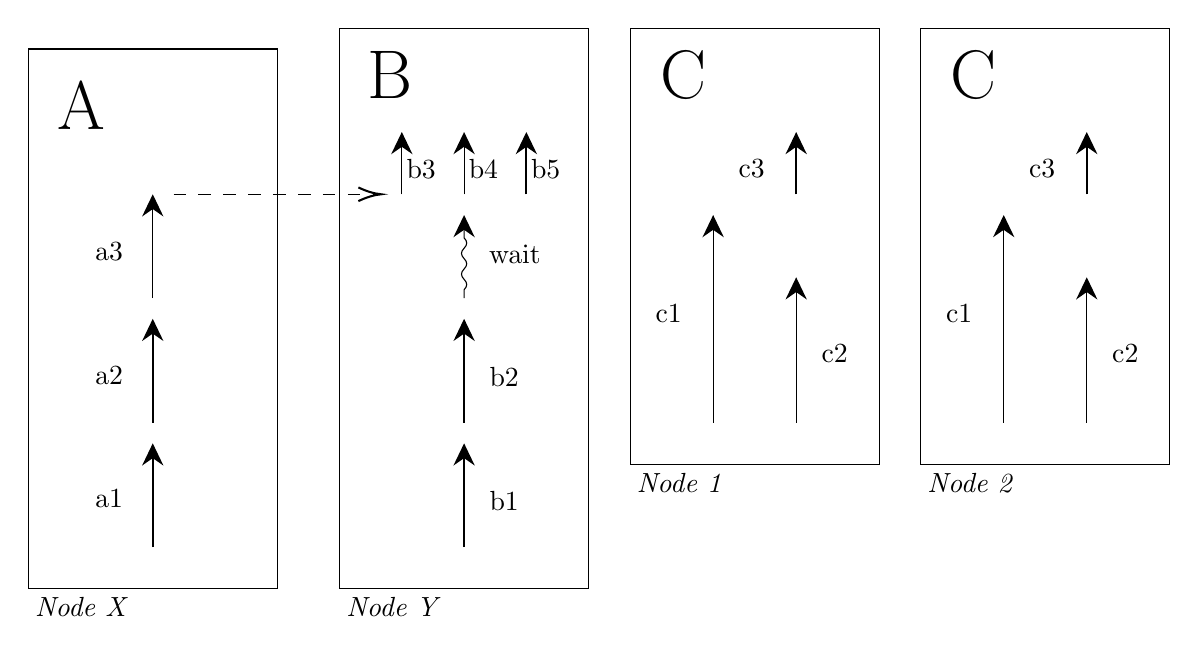
\begin{tikzpicture}[x=0.75pt,y=0.75pt,yscale=-1,xscale=1]
%uncomment if require: \path (0,320); %set diagram left start at 0, and has height of 320

%Straight Lines [id:da27430706126077264] 
\draw [color={rgb, 255:red, 0; green, 0; blue, 0 }  ,draw opacity=1 ][fill={rgb, 255:red, 255; green, 0; blue, 0 }  ,fill opacity=1 ][line width=0.75]    (80,263.5) -- (80,216.5) ;
\draw [shift={(80,213.5)}, rotate = 450] [fill={rgb, 255:red, 0; green, 0; blue, 0 }  ,fill opacity=1 ][line width=0.08]  [draw opacity=0] (10.72,-5.15) -- (0,0) -- (10.72,5.15) -- (7.12,0) -- cycle    ;
%Straight Lines [id:da18541775456344745] 
\draw [color={rgb, 255:red, 0; green, 0; blue, 0 }  ,draw opacity=1 ][fill={rgb, 255:red, 144; green, 19; blue, 254 }  ,fill opacity=1 ][line width=0.75]    (80,203.5) -- (80,156.5) ;
\draw [shift={(80,153.5)}, rotate = 450] [fill={rgb, 255:red, 0; green, 0; blue, 0 }  ,fill opacity=1 ][line width=0.08]  [draw opacity=0] (10.72,-5.15) -- (0,0) -- (10.72,5.15) -- (7.12,0) -- cycle    ;
%Straight Lines [id:da9191051295157292] 
\draw    (80,143.5) -- (80,96.5) ;
\draw [shift={(80,93.5)}, rotate = 450] [fill={rgb, 255:red, 0; green, 0; blue, 0 }  ][line width=0.08]  [draw opacity=0] (10.72,-5.15) -- (0,0) -- (10.72,5.15) -- (7.12,0) -- cycle    ;
%Straight Lines [id:da565354971469586] 
\draw [color={rgb, 255:red, 0; green, 0; blue, 0 }  ,draw opacity=1 ][line width=0.75]    (230,263.5) -- (230,216.5) ;
\draw [shift={(230,213.5)}, rotate = 450] [fill={rgb, 255:red, 0; green, 0; blue, 0 }  ,fill opacity=1 ][line width=0.08]  [draw opacity=0] (10.72,-5.15) -- (0,0) -- (10.72,5.15) -- (7.12,0) -- cycle    ;
%Straight Lines [id:da6700429327448342] 
\draw [color={rgb, 255:red, 0; green, 0; blue, 0 }  ,draw opacity=1 ][line width=0.75]    (230,203.5) -- (230,156.5) ;
\draw [shift={(230,153.5)}, rotate = 450] [fill={rgb, 255:red, 0; green, 0; blue, 0 }  ,fill opacity=1 ][line width=0.08]  [draw opacity=0] (10.72,-5.15) -- (0,0) -- (10.72,5.15) -- (7.12,0) -- cycle    ;
%Straight Lines [id:da28075371980457553] 
\draw [color={rgb, 255:red, 0; green, 0; blue, 0 }  ,draw opacity=1 ]   (200,93.5) -- (200,66.5) ;
\draw [shift={(200,63.5)}, rotate = 450] [fill={rgb, 255:red, 0; green, 0; blue, 0 }  ,fill opacity=1 ][line width=0.08]  [draw opacity=0] (10.72,-5.15) -- (0,0) -- (10.72,5.15) -- (7.12,0) -- cycle    ;
%Straight Lines [id:da9441221295165446] 
\draw [color={rgb, 255:red, 0; green, 0; blue, 0 }  ,draw opacity=1 ]   (230,93.5) -- (230,66.5) ;
\draw [shift={(230,63.5)}, rotate = 450] [fill={rgb, 255:red, 0; green, 0; blue, 0 }  ,fill opacity=1 ][line width=0.08]  [draw opacity=0] (10.72,-5.15) -- (0,0) -- (10.72,5.15) -- (7.12,0) -- cycle    ;
%Straight Lines [id:da3794379224544834] 
\draw [color={rgb, 255:red, 0; green, 0; blue, 0 }  ,draw opacity=1 ][line width=0.75]    (260,93.5) -- (260,66.5) ;
\draw [shift={(260,63.5)}, rotate = 450] [fill={rgb, 255:red, 0; green, 0; blue, 0 }  ,fill opacity=1 ][line width=0.08]  [draw opacity=0] (10.72,-5.15) -- (0,0) -- (10.72,5.15) -- (7.12,0) -- cycle    ;
%Straight Lines [id:da13857817807873274] 
\draw [color={rgb, 255:red, 0; green, 0; blue, 0 }  ,draw opacity=1 ]   (350,203.5) -- (350,106.5) ;
\draw [shift={(350,103.5)}, rotate = 450] [fill={rgb, 255:red, 0; green, 0; blue, 0 }  ,fill opacity=1 ][line width=0.08]  [draw opacity=0] (10.72,-5.15) -- (0,0) -- (10.72,5.15) -- (7.12,0) -- cycle    ;
%Straight Lines [id:da18881367347259226] 
\draw [color={rgb, 255:red, 0; green, 0; blue, 0 }  ,draw opacity=1 ]   (390,203.5) -- (390,136.5) ;
\draw [shift={(390,133.5)}, rotate = 450] [fill={rgb, 255:red, 0; green, 0; blue, 0 }  ,fill opacity=1 ][line width=0.08]  [draw opacity=0] (10.72,-5.15) -- (0,0) -- (10.72,5.15) -- (7.12,0) -- cycle    ;
%Straight Lines [id:da5578630098708864] 
\draw [color={rgb, 255:red, 0; green, 0; blue, 0 }  ,draw opacity=1 ][line width=0.75]    (390,93.5) -- (390,66.5) ;
\draw [shift={(390,63.5)}, rotate = 450] [fill={rgb, 255:red, 0; green, 0; blue, 0 }  ,fill opacity=1 ][line width=0.08]  [draw opacity=0] (10.72,-5.15) -- (0,0) -- (10.72,5.15) -- (7.12,0) -- cycle    ;
%Straight Lines [id:da19300882959893817] 
\draw  [dash pattern={on 4.5pt off 4.5pt}]  (90,93.5) -- (188,93.5) ;
\draw [shift={(190,93.5)}, rotate = 180] [color={rgb, 255:red, 0; green, 0; blue, 0 }  ][line width=0.75]    (10.93,-3.29) .. controls (6.95,-1.4) and (3.31,-0.3) .. (0,0) .. controls (3.31,0.3) and (6.95,1.4) .. (10.93,3.29)   ;
%Straight Lines [id:da8425704792181163] 
\draw [color={rgb, 255:red, 0; green, 0; blue, 0 }  ,draw opacity=1 ]   (490,203.5) -- (490,106.5) ;
\draw [shift={(490,103.5)}, rotate = 450] [fill={rgb, 255:red, 0; green, 0; blue, 0 }  ,fill opacity=1 ][line width=0.08]  [draw opacity=0] (10.72,-5.15) -- (0,0) -- (10.72,5.15) -- (7.12,0) -- cycle    ;
%Straight Lines [id:da4623771258590563] 
\draw [color={rgb, 255:red, 0; green, 0; blue, 0 }  ,draw opacity=1 ]   (530,203.5) -- (530,136.5) ;
\draw [shift={(530,133.5)}, rotate = 450] [fill={rgb, 255:red, 0; green, 0; blue, 0 }  ,fill opacity=1 ][line width=0.08]  [draw opacity=0] (10.72,-5.15) -- (0,0) -- (10.72,5.15) -- (7.12,0) -- cycle    ;
%Straight Lines [id:da01593649548581877] 
\draw [color={rgb, 255:red, 0; green, 0; blue, 0 }  ,draw opacity=1 ][line width=0.75]    (530,93.5) -- (530,66.5) ;
\draw [shift={(530,63.5)}, rotate = 450] [fill={rgb, 255:red, 0; green, 0; blue, 0 }  ,fill opacity=1 ][line width=0.08]  [draw opacity=0] (10.72,-5.15) -- (0,0) -- (10.72,5.15) -- (7.12,0) -- cycle    ;
%Straight Lines [id:da11733369284313999] 
\draw    (230,106.5) -- (230,114.5) .. controls (231.67,116.17) and (231.67,117.83) .. (230,119.5) .. controls (228.33,121.17) and (228.33,122.83) .. (230,124.5) .. controls (231.67,126.17) and (231.67,127.83) .. (230,129.5) .. controls (228.33,131.17) and (228.33,132.83) .. (230,134.5) .. controls (231.67,136.17) and (231.67,137.83) .. (230,139.5) -- (230,143.5) -- (230,143.5) ;
\draw [shift={(230,103.5)}, rotate = 90] [fill={rgb, 255:red, 0; green, 0; blue, 0 }  ][line width=0.08]  [draw opacity=0] (10.72,-5.15) -- (0,0) -- (10.72,5.15) -- (7.12,0) -- cycle    ;
%Shape: Rectangle [id:dp6987570624593641] 
\draw   (20,23.5) -- (140,23.5) -- (140,283.5) -- (20,283.5) -- cycle ;
%Shape: Rectangle [id:dp026922254453187522] 
\draw   (170,13.5) -- (290,13.5) -- (290,283.5) -- (170,283.5) -- cycle ;
%Shape: Rectangle [id:dp3707896533993156] 
\draw   (310,13.5) -- (430,13.5) -- (430,223.5) -- (310,223.5) -- cycle ;
%Shape: Rectangle [id:dp19211708743148737] 
\draw   (450,13.5) -- (570,13.5) -- (570,223.5) -- (450,223.5) -- cycle ;

% Text Node
\draw (45.5,51) node  [font=\Huge] [align=left] {A};
% Text Node
\draw (194.5,36) node  [font=\Huge] [align=left] {B};
% Text Node
\draw (335.5,36) node  [font=\Huge] [align=left] {C};
% Text Node
\draw (475.5,36) node  [font=\Huge] [align=left] {C};
% Text Node
\draw (254.5,122.5) node   [align=left] {wait};
% Text Node
\draw (51,234.5) node [anchor=north west][inner sep=0.75pt]   [align=left] {a1};
% Text Node
\draw (51,175.5) node [anchor=north west][inner sep=0.75pt]   [align=left] {a2};
% Text Node
\draw (51,115.5) node [anchor=north west][inner sep=0.75pt]   [align=left] {a3};
% Text Node
\draw (241,235.5) node [anchor=north west][inner sep=0.75pt]   [align=left] {b1};
% Text Node
\draw (241,175.5) node [anchor=north west][inner sep=0.75pt]   [align=left] {b2};
% Text Node
\draw (201,75.5) node [anchor=north west][inner sep=0.75pt]   [align=left] {b3};
% Text Node
\draw (231,75.5) node [anchor=north west][inner sep=0.75pt]   [align=left] {b4};
% Text Node
\draw (261,75.5) node [anchor=north west][inner sep=0.75pt]   [align=left] {b5};
% Text Node
\draw (321,145.5) node [anchor=north west][inner sep=0.75pt]   [align=left] {c1};
% Text Node
\draw (401,164.5) node [anchor=north west][inner sep=0.75pt]   [align=left] {c2};
% Text Node
\draw (361,75.5) node [anchor=north west][inner sep=0.75pt]   [align=left] {c3};
% Text Node
\draw (461,145.5) node [anchor=north west][inner sep=0.75pt]   [align=left] {c1};
% Text Node
\draw (541,164.5) node [anchor=north west][inner sep=0.75pt]   [align=left] {c2};
% Text Node
\draw (501,75.5) node [anchor=north west][inner sep=0.75pt]   [align=left] {c3};
% Text Node
\draw (22,286.5) node [anchor=north west][inner sep=0.75pt]   [align=left] {\textit{Node X}};
% Text Node
\draw (172,286.5) node [anchor=north west][inner sep=0.75pt]   [align=left] {\textit{Node Y}};
% Text Node
\draw (312,226.5) node [anchor=north west][inner sep=0.75pt]   [align=left] {\textit{Node 1}};
% Text Node
\draw (452,226.5) node [anchor=north west][inner sep=0.75pt]   [align=left] {\textit{Node 2}};


\end{tikzpicture}
}
        \end{minipage}
      } \label{fig:intra-comp-tasks}
    }
    \caption{Examples to illustrate the four parallelism levels
      considered in this paper}
    \label{fig:parlevels}
  \end{center}
\end{figure*}

One can note that presented metrics for both SE and parallelism are
procedural-oriented as they consider \emph{tasks} and not
\emph{resources}, thus excluding \puppet or \salt for instance. While
being an approach with great advantages, declarative approaches are
not considered in this paper.

\paragraph{Formalism}
The last metric considered to compare the related work is the
existence of a formal model for each commissioning solution. Indeed,
we claim that studying formally commissioning models and their
operational semantics is of high importance to open the door to
verification and safety in commissionings and by extension
reconfigurations. For instance, even if this contribution is not
presented in this paper, the formal model \mad has been
successfully used to verify safety properties on distributed software
commissionings by model checking~\cite{coullon:hal-02323641}.

%----------------------------
\subsection{Description and comparison of the related work}
% ----------------------------

Among the plethora of distributed software commissioning solutions, we
have selected a subpart of them for a deeper comparison. According to
the classification of Section~\ref{sec:context}, we have selected: two
\emph{coding} or scripting solutions, \shell and \fractal; three
procedural-oriented solutions of the \emph{software configuration}
class, \ansible, \deployware and \aeolus; two solutions of the
\emph{infrastructure definition} class, \juju and \tosca; and finally
one \emph{orchestration} solution, \kubernetes. In this selection we
have taken a particular attention to select both production tools and
academic contributions. Moreover, we have selected production tools
having a significant opensource community.

% Shell-scripts
\paragraph{Shell scripts}
The traditional way operators automate software commissioning is by
transcribing the actions and configurations from READMEs and tutorials
into a sequence of commands in \shell scripts. On the one hand, those
scripts are written with low-level imperative languages, and with good
programming skills, it is possible to express complex workflows (\eg
idempotency, parallelism, remote actions using \textsc{SSH}). For
instance, parallelism can be managed by combining command execution in
the background (\eg using the control operator \& in \bash) and
synchronisation commands like \emph{wait}. On the other hand, as the
system grows, any custom script becomes error-prone, unpredictable,
hard to understand and to maintain. \shell scripts lack of software
engineering aspects and there is no framework to express modules nor
tasks and their dependencies thus making separation of concerns a very
tricky work. In Table~\ref{tab:comparison} we indicate that each
metric introduced could potentially be implemented manually by using
\shell. Of course, such mechanisms are difficult to implement, error
prone, and time consuming.
% devstack is a set of shell script to deploy OpenStack on a single machine

\paragraph{Fractal}
Component-based software engineering (CBSE) is a domain that enhances
(distributed) software implementation by dealing with code re-use,
separations of concerns, and composability (thus maintainability) of
software codes~\cite{Szyperski:2002:CSB:515228}. A component-based
application is composed of a set of component instances connected
together. Such composition of components is called an
\emph{assembly}. A component is a black box that implements an
independent functionality of an application, and which interacts with
other components through well defined interfaces, called \emph{ports}.
Ports are used to decouple the component internals from its
interface. For instance, a port can be used to declare that the
component either provides a service ---in this case the port is
attached to an internal method--- or use a service from another
component. Many component models focus on the implementation of the
functionalities and
interfaces~\cite{corba:omg06,Blair2009,baude:hal-01001043,Bernholdt01052006,bigot:inria-00388508,Coullon2017}
of components, rather than on their commissioning. A few component
models have contributed to commissioning issues. In the Object
Management Group's (OMG) specification~\cite{ccmdeploy:omg06}, the
commissioning model is rigid and fixed by the model. In
\fractal~\cite{Blair2009} and its evolutions GCM and
GCM/ProActive~\cite{baude:hal-01001043}, the control of a component
(\eg its commissioning) is decoupled from its functionalities into a
so called \emph{membrane} which is itself described as a component
assembly written in java. The membrane is handled by the \fractal
runtime but the sub-assembly and its associated codes are entirely
left to the user. That is why in Table~\ref{tab:comparison}, metrics
not natively supported by \fractal can be handled manually using
java. Both \emph{sparation of concerns} and \emph{inter-comp} are well
handled by \fractal thanks to the notion of port (dependencies within
the component or with an external component) adapted to the
membrane. One can note that only \fractal components commissionings
can be written in the membrane, thus if writing the commissioning of
existing modules they have to be encapsulated in a \fractal component.

% Deployware
\paragraph{Deployware}
\citeauthor{flissi2008ccgrid} proposed \deployware (DW) as a research
effort to distributed software commissioning in the context of Grid
computing~\cite{flissi2008ccgrid}. Its implementation is based on the
\fractal component model. A component is called a \emph{Personality}
and is associated to a fixed set of commissioning actions (\ie
install, configure, start, manage, stop, unconfigure and uninstall),
which can be considered as a fix set of \emph{tasks}.  Each action
describes a sequence of tasks, written with a specific high-level
language that uses pre-defined instructions (\eg execute command, copy
a file). While there is no notion of component ports, it is possible
to express dependencies between components to initiate automatic
coordination. For instance, when the operator triggers the action
"install" on a component, the same action is triggered recursively to
its dependencies. As theyr are not entirely controllable by the user,
metrics \emph{tasks}, \emph{SIMH} and \emph{inter-comp} are considered
as partially supported by \deployware. Finally, as \deployware is
based on \fractal and as a formal effort have been done on \fractal,
the formal aspect of \deployware is considered partially supported.

% Ansible
\paragraph{Ansible}
For the DevOps that are used to shell-scripts, \ansible has become a
popular configuration management tool since it relies on a simple
syntax written in YAML and does not require agents on administrated
servers. Tasks are indeed managed using only \textsc{SSH} and
\textsc{Python} which are commonly installed on every Linux
distributions.  In comparison, similar tools like \chef, \puppet or
\cfengine not only require at least a slight understanding of Ruby or
a custom language to get started, but they are built on an agent-based
architecture and requires prior agent commissioning on remote hosts.
\ansible features software engineering aspects like separation of
concerns by defining the notion of \emph{roles} which can be seen as
software components.  Each role contains a set of files that describe
a sequence of tasks. To define a composition, a specific file called
an \ansible \emph{playbook} is used for mapping the desired roles to
the groups of nodes they will be applied to. Those groups of nodes are
defined in a separate file called the \emph{inventory}. When \ansible
is triggered, roles and their related tasks are sequentially executed
to the associated groups of nodes. While tasks declarations are indeed
manages sequentially, each task is executed in parallel when mapped to
multiple remote hosts thus leading to the \emph{SIMH} metric.
Typically, an operator who wants to commission an \apache web server
and a \mysql database would download two roles from Ansible Galaxy and
register them in an playbook. Since \ansible triggers roles in a
sequential manner, if the operator is not aware that the database must
be commissioned before the web server, she could make a mistake in the
order of the roles she declared. This aspect makes the
\emph{separation of concerns} metric only partially
supported. Finally, as one of the possible type of tasks in \ansible
is the execution of a \shell command, any script could be executed as
a task thus making possible to handle manually the \emph{intra-comp-tasks}
parallelism level.

% Tasks are declared in an imperative way, however, Ansible relies heavily on
% declarative modules, most of which ensure task idempotency (operations are run
% once even if called multiple times).

% Aeolus
\paragraph{Aeolus}
\citeauthor{dicosmo2014ic} proposed \aeolus: a formal component-based
model for the cloud~\cite{dicosmo2014ic}. Their component model
captures the internal states of a component commissioning process
thanks to a finite state machine. Each state can be connected to use,
provide, or conflict ports to declare dependencies between the
commissioning steps of different components. Hence, such ports enable
the coordination of the global deployment process.

% Juju
\paragraph{Juju}
Canonical has developed their own software commissioning solution:
\juju (\url{https://jujucharms.com/}) which aims at commissioning any
kind of application on top of different cloud providers (\eg AWS,
OpenStack), and on multiple types of resources (container, VM or
bare-metal). Its concepts are close to component models. Software
modules are packaged as \juju \emph{charms} which describe the
software commissioning steps through a set of scripts called
\emph{hooks}. Operators define their composition in a specific file
called \emph{bundle} in which they declare the desired charms with
their \emph{relations}. A relation is an element declared between two
charms and used for component synchronization (by triggering hooks)
and data sharing at runtime, similarly to component ports. As the
concepts behind \juju are very close to the one of \aeolus the same
metrics are available except the formal aspect.
% good soc, download charms and run juju deploy

\paragraph{TOSCA}
The \emph{Topology and Orchestration Specification for Cloud
  Applications} (TOSCA) is another component-oriented model that
partially addresses the commissioning of its
components. TOSCA~\cite{tosca:web,10.1007/978-3-319-74781-1_33} is a
standardization effort from OASIS to describe Cloud applications,
their components and their deployment artifacts, using standard
languages (\ie XML, YAML). A TOSCA description (or template)
corresponds to a graph where nodes represent TOSCA resources
(e.g. software components, virtual machines, physical servers), and
where edges represent the relations between those nodes. Artifacts (of
any type: scripts, executable etc.) can be added to TOSCA descriptions
in a CSAR (Cloud Service ARchive) to detail commissioning steps. Those
commissioning steps can thus be customized by the developper but there
is no model and guarantees associated to them. Thus \emph{tasks} and
\emph{intra-comp-tasks} metrics could handled manually by the user. As
there is no way to declare dependencies between artifacts of
components the \emph{inter-taks} metric is not supported, however,
relations between components make both \emph{SIMH} and
\emph{inter-comp} metrics theoretically available in \tosca. No
information have been found on the complete support of these metrics
in \tosca implementations~\cite{cloudify:web,opentosca:web}. Finally,
come efforst have been done to formally define the \tosca
standard~\cite{tosca:web}.

% Kubernetes
\paragraph{Kubernetes}
Initiated by Google, \kubernetes (K8S) is a popular framework to
commission distributed software in the form of micro-services that are
packaged as a hierarchy of Docker containers and \emph{pods}. A
software component in \kubernetes is thus defined as Docker
container. Such components have no port to manage coordination, and
its internals is fixed since containers can only be started and
stopped. As a consequence, the commissioning process is
error-prone. For instance, a web server can be started before the
required database and thus fails. For this reason, the metric
\emph{inter-comp} is considered as partially supported.
% depend_on exists but limited to "container is started"
% synchronization is possible but must be managed by internal script and not managed by k8s
% good soc, download containers and run k8s deploy but without synchonization,
    % commissioning is error-prone

\begin{table*}[tp]
  \centering
  \small
  

% \begin{tabular}{cl|cccccc}
%     \toprule
%     & & Shell & Ansible & DW & K8S & Juju & Aeolus \\
%     \midrule
%     %\rowcolor{gray!15}
%     \multirow{3}{*}{\STAB{\rotatebox[origin=c]{90}{Parallel}}}
%     & node    & \checkmark & \checkmark & \checkmark & \checkmark & \checkmark & \checkmark \\
%     & inter   & \checkmark &   &   &   & \checkmark & \checkmark \\
%     %\rowcolor{gray!15}
%     & intra   & \checkmark &   &   &   &   &   \\
%     \midrule
%     \multirow{2}{*}{\STAB{\rotatebox[origin=c]{90}{SE}}}
%     & module  &   & \checkmark & \checkmark & \checkmark & \checkmark & \checkmark \\
%     %\rowcolor{gray!15}
%     & ports   &   &   &   &   & \checkmark & \checkmark \\
%     \bottomrule
% \end{tabular}

% \newcolumntype{g}{>{\columncolor{gray!15}}c}
% \begin{tabular}{cl|gc|gcgc|gc|g}
%   \toprule
%   \rowcolor{white}
%   & & \multicolumn{2}{c|}{\textit{Coding}} & \multicolumn{4}{c|}{\textit{Software configuration}} & \multicolumn{2}{c|}{\textit{Provisioning}} & \textit{Orchestration} \\
%   \midrule
%   & & \shell & \fractal & \textbf{\ansible} & \puppet & \deployware & \textbf{\aeolus} & \juju & \tosca & \kubernetes \\
%   & & & \cite{} & \cite{} & \cite{} & \cite{} & \cite{} & \cite{} & \cite{} & \cite{} \\ 
%   \midrule
%   \multirow{4}{*}{\STAB{\rotatebox[origin=c]{90}{Soft. eng.}}}
%   & components & M & \checkmark & \checkmark & \checkmark & \checkmark & \checkmark & \checkmark & \checkmark & \checkmark \\
%   & tasks & M & M & \checkmark & M & (\checkmark) & \checkmark & \checkmark & M & \\
%   & resources & M & M & & \checkmark & & & & \checkmark & \\
%   & sep. of con. & M & (\checkmark) & (\checkmark) & \checkmark & \checkmark & (\checkmark) & (\checkmark) & \checkmark & \checkmark \\
%   \midrule
%   \multirow{5}{*}{\STAB{\rotatebox[origin=c]{90}{Parallelism}}}
%   & SIMH & M & (\checkmark) & \checkmark & \checkmark & (\checkmark) & \checkmark & \checkmark & (\checkmark)& \checkmark\\
%   & inter-comp & M & (\checkmark) & & & (\checkmark) & \checkmark & \checkmark & (\checkmark)& (\checkmark)\\
%   & inter-task & M & M & & & & \checkmark & \checkmark & & \\
%   & inter-resource & M & M & & (\checkmark) & & & & (\checkmark) & \\
%   & intra-task & M & M & M & M & M & M & M & M & \\
%   \midrule
%   & formal & & \checkmark & & & (\checkmark) & \checkmark & & \checkmark & \\
%   \midrule
%   & score & 9 & 17 & 11 & 14 & 14 & 20 & 17 & 18 & 11\\
%     \bottomrule
% \end{tabular}

% without resources and puppet

\newcolumntype{g}{>{\columncolor{gray!15}}c}
\begin{tabular}{cl|gc|gcg|cg|c}
  \toprule
  \rowcolor{white}
  & & \multicolumn{2}{c|}{\textit{Coding}} & \multicolumn{3}{c|}{\textit{Software configuration}} & \multicolumn{2}{c|}{\textit{Infrastructure}} & \textit{Orchestration} \\
  \midrule
  & & \shell & \fractal & \deployware & \ansible & \aeolus & \juju & \tosca & \kubernetes \\
  & & & \cite{Baude,Blair2009,baude:hal-01001043} & \cite{flissi2008ccgrid} & \cite{ansible:web} & \cite{dicosmo:hal-01233489,dicosmo2014ic,zwolakowski:tel-01172022} & \cite{juju:web} & \cite{tosca:web,brogi2018,7561358,8599581} & \cite{kubernetes:web,43826} \\ 
  \midrule
  \multirow{3}{*}{\STAB{\rotatebox[origin=c]{90}{SE}}}
  & components & M & \checkmark & \checkmark & \checkmark & \checkmark & \checkmark & \checkmark & \checkmark \\
  & tasks & M & M & (\checkmark) & \checkmark & \checkmark & (\checkmark) & M & - \\
  & sep. of con. & M & \checkmark & \checkmark & (\checkmark) & (\checkmark) & (\checkmark) & \checkmark & \checkmark \\
  \midrule
  \multirow{4}{*}{\STAB{\rotatebox[origin=c]{90}{Parallel}}}
  & SIMH & M & \checkmark & (\checkmark) & \checkmark & \checkmark & \checkmark & (\checkmark)& \checkmark\\
  & inter-comp & M & \checkmark & (\checkmark) & - & \checkmark & \checkmark & (\checkmark)& (\checkmark)\\
  & inter-comp-tasks & M & M & - & - & \checkmark & (\checkmark) & - & - \\
  & intra-comp-tasks & M & M & M & M & M & M & M & - \\
  \midrule
  & formal & - & \checkmark & (\checkmark) & - & \checkmark & - & \checkmark & -\\
  \midrule
  & score & 7 & 18 & 15 & 12 & 21 & 16 & 15 & 11\\
    \bottomrule
\end{tabular}



  \caption{Comparison of commissioning solutions based on aspects
  regarding parallelism (performance) and software engineering (SE).}
  \label{tab:comparison}
\end{table*}

%----------------------------
\subsection{Discussions}
%----------------------------
% 3. discussion
% - flexibility vs automation vs formal
% - separation of concerns
% - intra-task parallelism
% - performance model and formal

In the previous section, eight different related works have been
compared according to software engineering metrics, parallelism
metrics and one metric regarding the formal definition of the
considered solution. Table~\ref{tab:comparison} resumes this
comparison and raises a few key points that we discuss in the
following.

As usual when working on programming languages, the existing
tools illustrate the difficult trade-off between flexibility and
automation. On the one hand, when the tool is highly programmable,
developers have the ability to manage their own code organization and
to handle any kind of software engineering or efficiency property. For
instance, by using \shell, any of the introduced metrics could be
handled. However, each of them would have to be hand-coded which is
difficult and error prone. On the other hand, some existing solutions
such as \deployware and \juju restrict the internal commissioning
behavior of components to a fix set of actions (\eg install,
configure, start). Such choice has the advantage of guaranteeing the
full control of the automated parallelism level but also restrict
potential optimizations due to the specificity of each component and
the interactions between components and their tasks.

One can note that \aeolus is the solution with the highest score
regarding the introduced metrics. Indeed, \aeolus combines advantages
of component models to structure the code of software commissionings
and enhance its separation of concerns, while introducing an
additional way to model the internal commissioning behavior of each
component through tasks. It seems that \aeolus offers a good trade-off
between flexibility and automation. However, while offering the best
combination of metrics, \aeolus partially handle separation of
concerns between components.

Furthermore, one can note that no existing solution offers a full
support for \emph{intra-comp-tasks} parallelism level. Actually, if a few
existing solutions already offer a way to model the internal
commissioning behavior of each component by using tasks, dependencies
between those tasks are limited to a sequential imperative order thus
making \emph{intra-comp-tasks} parallelism impossible. Such parallelism
could be handled manually by some of the existing tools, however such
parallel aspects are difficult to implement and error prone, thus they
should be handled automatically.

If introducing more parallelism opens up additional performance
capabilities, it also introduces more complexity for the user. For
this reason, formalizing the commissioning solution is of high
importance to guarantee properties such as attainability of
commissionings.

\begin{tcolorbox}[enhanced,attach boxed title to top left={yshift=-3mm,yshifttext=-1mm},
  colback=black!5!white,colframe=black!30,colbacktitle=black!60,
  title=Contribution,fonttitle=\bfseries,
  boxed title style={size=small,colframe=black!60,boxrule=0.2mm},
  boxrule=0.2mm]
  \mad is a formal component model inpired by \aeolus that enhances
  the automation, the separation of concerns and the parallelism level
  of distributed software commissionings.
\end{tcolorbox}

% One further aspect of the level of programmability provided by commissioning
% tools. When the tool is highly programmable, developers have the ability to
% manage their own code organization. This is an important aspect to finely
% express what can be executed in parallel (thus it impacts performance). For
% instance \deployware and \juju limit the internals of their modules to a
% predefined set of actions (eg config, install) while such actions might contain
% instructions that can be declared parallelable.
% %
% Our solution differs by letting developers abstract a set of instructions in the
% form of transitions. Transitions can be expressed in parallel, and their
% synchronisation is declared using states.
% %high programmable can also  improve maintainability by isolating specfic code
% %in a transition.

% Finally, a desired feature for distributed software commissioning is automation.
% Typically an operator should download the desired modules to compose a
% distributed software, instantiate and connect them through their ports, then run
% the commissioning process. This aspect requires an operational semantic to
% express how the commissioning process automatically progresses with respect to
% inter and intra-component dependencies. For instance, \aeolus, which supports
% only inter-component parallelism, is a component-based model that relies on
% states and transitions to manage inter-component dependencies. However, since
% the model lacks an operational semantic, each operation is planned and executed
% by an external scheduler. In this work, one of our contribution is to provide a
% operational semantic which drives the execution of the distributed software
% commissioning, and will be explained in \cref{subsec:operational_semantics}.

% As depicted in~\cref{tab:comparison}, we can conclude from this analysis that
% individually, none of the above attempts adequately provide a commissioning tool
% which can express both a high-degree of parallelism and feature software
% engineering aspects like separation of concerns.
% In the rest of this paper, we define \mad, our contribution which is inspired by
% \aeolus as a component-based model and relies on modules and ports to express all
% the parallelism levels described above. In the rest of the paper, we will
% focus the comparison of our solution with \ansible and \aeolus, since the former
% is widely used in production, while the second is a research effort that
% provides most of the above features.

